%   Filename    : chapter_4.tex 
\chapter{Results and Discussions}
%This chapter  presents the results or  the system  of your SP.  Include screenshots, tables, or graphs and provide the discussion of results.
This chapter discusses the results and analysis of the study. As specified, the study focuses on building an animal rescue system that implements gamification and login features for the Aklan Animal Rescue and Rehabilitation Center in Kalibo, Aklan. 

\section{Results}

The state of the current web-based systems of animal rescue centers are straightforward
and simple. It is important to make it as user-friendly as possible so that
it would be easier for the users to engage in the system. But simplicity does
not always mean the more users would engage on it. Gamification integrates the
“human” to the system and is considered in designing that motivates more
users to take part in using the system.

There are general ways in finding out what motivates the user of an animal
rescue center,the researchers used that motivation to drive the users to do certain actions they would not normally do. The specific motivation for a web-based animal
rescue system that the researchers used is a virtual pet that evolves when it will reach a certain
level. The way to gain experience points to level up is by doing actions in a typical
animal rescue system like donating, adopting, and volunteering.

\subsection{Sign-up Page}


%--- the following example shows how to include a figure in PNG format
\begin{figure}[h]                %-- use [t] to place figure at top, [b] to place at the bottom, [h] for here
	\centering                    %-- use this to center the figure
	
\includegraphics{SUP.png}      %-- include image file named as "disneychart.png" 
	\caption{The sign up page shows a form where the user will input credentials
		such as username, email, and password. These credentials are used to make an
		account for the user to access exclusive features such as the virtual pet. The user
		can also use third-party services to provide necessary information for signing up
		such as Facebook and Google.}
	\label{fig:disneystock}
	
\end{figure}

\subsection{Login Page}

%--- the following example shows how to include a figure in PNG format
\begin{figure}[h]                %-- use [t] to place figure at top, [b] to place at the bottom, [h] for here
	\centering                    %-- use this to center the figure
	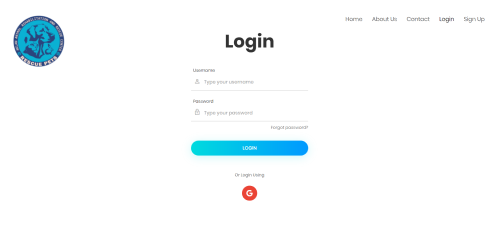
\includegraphics{LogPage.png}      %-- include image file named as "disneychart.png" 
	\caption{The login page allows the user that has already an existing account
		to sign in to the system. The user is asked to input the username and password
		or either use third party services such as Facebook and Google to login.}
	\label{fig:disneystock}
\end{figure}

\subsection{Home Page}

%--- the following example shows how to include a figure in PNG format
\begin{figure}[h]                %-- use [t] to place figure at top, [b] to place at the bottom, [h] for here
	\centering                    %-- use this to center the figure
	\includegraphics{Home Page.png}      %-- include image file named as "disneychart.png" 
	\caption{The homepage of the system consists of three sub-pages: the main
	page, the information page, and the contacts page. Each page can be accessed
	either by scrolling or aside clicking each corresponding button at the navigation
	bar above the home page. In the navigation bar. The main page has a “Join
	Now” button where users can create an account and sign up.}
	\label{fig:disneystock}
\end{figure}

\subsection{Profile {Page}}

%--- the following example shows how to include a figure in PNG format
\begin{figure}[h]                %-- use [t] to place figure at top, [b] to place at the bottom, [h] for here
	\centering                    %-- use this to center the figure
	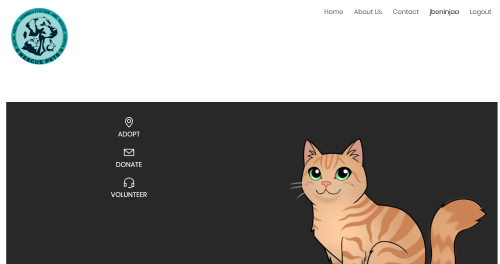
\includegraphics{Profile page.png}      %-- include image file named as "disneychart.png" 
	\caption{The homepage of the system consists of three sub-pages: the main
		page, the information page, and the contacts page. Each page can be accessed
		either by scrolling or aside clicking each corresponding button at the navigation
		bar above the home page. In the navigation bar. The main page has a “Join
		Now” button where users can create an account and sign up.}
	\label{fig:disneystock}
\end{figure}





